% Springer Nature manuscript for Signal, Image and Video Processing (SIViP)
\documentclass[iicol,pdflatex,sn-basic,Numbered]{sn-jnl}

\usepackage{graphicx}
\usepackage{amsmath,amssymb,amsfonts}
\usepackage{booktabs}
\usepackage{tabularx}
\usepackage{multirow}
\usepackage{url}

\raggedbottom

\begin{document}

\title[Fixed-budget local-patch risk routing]{Fixed-Budget Local-Patch Risk Routing for Industrial Anomaly Detection}

\author*[1]{\fnm{Jin} \sur{Huang}}\email{614938561@qq.com; \href{https://orcid.org/0009-0005-7489-2018}{ORCID: 0009-0005-7489-2018}}
\author[2]{\fnm{Qisen} \sur{Gao}}\email{1350728839@qq.com}

\affil*[1]{\orgname{Guangxi Vocational Normal University}, \orgaddress{\city{Nanning}, \postcode{530007}, \state{Guangxi Zhuang Autonomous Region}, \country{China}}}
\affil[2]{\orgname{Gansu University of Political Science and Law}, \orgaddress{\city{Lanzhou}, \postcode{730070}, \state{Gansu}, \country{China}}}

\abstract{Industrial anomaly detection cannot always afford to run an expensive local detector on every image. We examine whether a low-cost local-patch probe can make better use of a fixed number of expensive evaluations than several simple allocation policies. The probe ranks images by layer-2 patch-to-normal-memory distance and sends the highest-risk 25\% to a layer-3 patch-memory path. Because every policy receives the same quota, differences between them reflect allocation quality rather than budget size. On MVTec AD (15 categories, three seeds), MPDD (6 categories, three seeds) and VisA (12 categories, three seeds), local-patch risk increased image-level area under the receiver operating characteristic curve (AUROC) over equal-count random allocation by +0.1249 (paired category-seed 95\% bootstrap confidence interval [0.0837, 0.1659]), +0.1166 ([0.0715, 0.1612]) and +0.0128 ([0.0081, 0.0171]), respectively. It also outperformed a nearest-patch-distance dispersion signal. The fast detector's own score was a harder baseline: it was close to local-patch risk on MVTec AD and stronger on MPDD and VisA. In a separate MVTec batch-one NVIDIA Compute Unified Device Architecture (CUDA) audit, the risk route had higher 95th-percentile (P95) latency than the full path. These results support local-patch risk as a fixed-budget allocation rule under the tested offline protocol, while ruling out claims of full-detector superiority, lower single-sample latency or stable online behaviour.}

\keywords{industrial anomaly detection, selective inference, risk routing, local patch memory, resource-aware inference}

\maketitle

\section{Introduction}\label{sec:introduction}

Industrial inspection systems process many normal products and a smaller, varied set of defective ones. Local feature extraction and memory comparison can reveal subtle defects, but running this path on every image assigns the same computational cost to easy and difficult cases. Lightweight global features cost less, yet they may miss small or localized defects. The resulting question is whether a cheap signal can identify the images that warrant local analysis.

Memory-based anomaly detection offers a natural test case. Patch-memory methods compare test descriptors with descriptors from normal training images, and both storage and nearest-neighbour search grow with the number of retained patches \cite{bergmann2019mvtec,defard2021padim,roth2022patchcore}. Related work has studied feature adaptation and synthetic anomaly features \cite{liu2023simplenet}, millisecond-level student-teacher inference \cite{batzner2024efficientad}, tiled high-resolution processing under memory constraints \cite{rolih2024divide}, and multimodal or prompt-based representations \cite{jeong2023winclip,li2024promptad,li2024promptadzero,costanzino2024multimodal}. Selective prediction and cascaded inference instead decide when to spend more computation. Their gains are difficult to interpret if one method sends more inputs to the expensive path than another \cite{geifman2017selective}, so a fair allocation comparison must hold that count fixed.

We test whether local-patch risk allocates a fixed quota of expensive evaluations better than matched-random selection. A low-resolution layer-2 probe ranks images without test labels, and a prescribed fraction enters a higher-resolution layer-3 patch-memory detector. The control selects the same number of images by uniform sampling without replacement. Thus, only the allocation rule changes; the fallback count, data split, feature path and evaluation unit remain fixed.

The comparison includes equal-count random selection, the fast detector's own anomaly score, and the dispersion of nearest patch-to-memory distances as an uncertainty signal. Each policy uses the same data, feature paths, seed and fallback count. The experiment therefore compares ranking signals at one budget rather than different amounts of computation.

This study contributes:
\begin{itemize}
\item a fixed-budget formulation that separates routing quality from full-detector accuracy in resource-constrained industrial inspection;
\item a lightweight layer-2 local-patch risk score evaluated under an exact fallback quota against equal-count random, fast-score and nearest-patch-distance dispersion baselines;
\item a matched-budget evaluation on three datasets and three seeds, with category-level robustness checks, MVTec results at 10/25/50\% budgets and a batch-one latency audit that identifies where local-patch risk is not the strongest policy.
\end{itemize}

The scope is limited to allocation under the tested offline quota. The route neither exceeds the full detector nor reduces single-sample P95 latency, and its behaviour changes with online batches and distribution shift.

\section{Related work}\label{sec:related}

\subsection{Industrial anomaly detection}
PatchCore stores representative normal patch features and scores queries by nearest-neighbour distance \cite{roth2022patchcore}, whereas PaDiM models patch distributions parametrically \cite{defard2021padim}. Other studies cover target-domain adaptation, zero- and few-shot vision-language features, supervised or semi-supervised industrial data, and memory-efficient high-resolution processing \cite{liu2023simplenet,jeong2023winclip,baitieva2024segad,rolih2024divide}. Reviews published in 2024 and 2025 summarize normal-only, few-shot, supervised, multimodal and efficiency-oriented settings \cite{tao2024deepindustrial,li2025survey,mao2025rethinks}. These methods are full-budget or alternative detector references, but they do not decide which images should enter an expensive path. We therefore evaluate routing separately from absolute detector accuracy.

\subsection{Selective prediction and resource-aware inference}
Selective prediction asks when a model should abstain or defer an input \cite{geifman2017selective}. A cascade first applies a cheap model, then sends selected cases to a more expensive one. In this setting, the number of expensive evaluations is a direct confound. Matching the random route to the risk quota isolates the ranking signal.

\subsection{Calibration and distribution shift}
Conformal methods provide finite-sample calibration guarantees under exchangeability \cite{vovk2005algorithmic,angelopoulos2023conformal}. Here, a conformal threshold is used only as a stress test. Its realized fallback rate drifted under the evaluated shift, so it cannot support a fixed-budget guarantee in this experiment.

\section{Method}\label{sec:method}

\subsection{Problem formulation}
Let $x$ denote an input image and $b\in(0,1)$ the target fraction allowed to use the full detector. The system has a fast path $f_s$, a local risk probe $r$ and a full path $f_f$. Its final score is
\begin{equation}
s_b(x)=\begin{cases}
s_f(x), & x\notin\mathcal{S}_b,\\
s_{\mathrm{full}}(x), & x\in\mathcal{S}_b,
\end{cases}
\end{equation}
where $\mathcal{S}_b$ is the selected set and $|\mathcal{S}_b|=\lceil bN\rceil$ for a test set of $N$ images. We compare the final score obtained from this risk-selected set with that from a uniformly sampled set of equal size.

\subsection{Fast and full feature paths}
The fast path resizes each image to $128\times128$ pixels and extracts layer-2 features from an ImageNet-pretrained ResNet-18. It normalizes the spatial descriptors and compares them with a memory bank built from normal training images. The full path uses $224\times224$ inputs and layer-3 local patch descriptors. Its anomaly score is the mean of the largest 10\% patch-to-memory nearest-neighbour distances. Both memory banks use only normal training images.

\subsection{Local-patch risk probe}
For a query image $x$, let $q_i(x)$ be its layer-2 spatial descriptors and let $\mathcal{M}_2$ be the normal layer-2 memory bank. The local risk score is
\begin{equation}
r(x)=\operatorname{MeanTop}_{5\%}\left(\left\{\min_{m\in\mathcal{M}_2}\lVert q_i(x)-m\rVert_2\right\}_i\right).
\end{equation}
The score averages the largest five percent of local distances, retaining sensitivity to spatially concentrated defects. We fixed this aggregation fraction before the formal cross-dataset comparison and use 1\%, 5\% and 10\% only for the ablation.

\subsection{Strict quota and matched-random control}
The risk route selects the $\lceil bN\rceil$ images with the largest $r(x)$ values. The matched-random controller draws exactly $\lceil bN\rceil$ indices without replacement and replaces their fast scores with the corresponding full scores. Both routes use the same images, normal memory banks, seeds, budget and evaluation code. Ranking and selection do not use test labels. Pairing is performed at the category-seed level, which is also the primary statistical unit; individual images and timing repetitions are not treated as independent units.

\subsection{Fast-score and uncertainty baselines}
The fast-score baseline ranks images by the fast detector's anomaly score, defined as the nearest-neighbour distance between a global layer-2 embedding and the normal-feature memory. It tests whether the local-patch probe adds information beyond a score that is already available. The uncertainty baseline uses the dispersion of nearest patch-to-memory distances, $u(x)=Q_{90}(d_i)-Q_{50}(d_i)$. This low-cost proxy differs from the top-$5\%$ mean used by the risk probe. Within each category-seed unit, both baselines select the same number of fallback images as the risk route. AUROC differences therefore cannot arise from unequal budgets.

\subsection{Online prefix controller}
We also evaluate an online prefix controller to separate strict transductive ranking from a setting closer to deployment. Images arrive in batches of 32. Using only current local-risk scores, each batch selects the number needed to maintain a cumulative 25\% quota. The controller does not inspect future scores or test labels. We report this analysis separately because route quality can change with batch composition and score shift.

\section{Experimental setup}\label{sec:setup}

\subsection{Datasets and protocol}
We evaluate MVTec AD (15 categories), MPDD (6 categories) and VisA (12 categories) \cite{bergmann2019mvtec,jezek2021mpdd,zou2022visa}. The formal 25\% analysis uses seeds 5, 17 and 29, yielding 45, 18 and 36 category-seed units, respectively. Every policy has the same fallback count within a category-seed unit. Thresholds and route definitions come from normal training or calibration data; test labels are reserved for evaluation. The MVTec budget analysis uses the same seeds at 10\%, 25\% and 50\%.

\subsection{Metrics and uncertainty}
Image-level AUROC is the primary metric, with recall at a 5\% false-positive rate as the low-FPR operating measure. We also report realized fallback rate, mean latency and P95 latency. Confidence intervals come from paired bootstrap resampling of category-seed units; timing repetitions are not independent experimental units. The primary comparison is local-patch risk versus matched-random selection under the same quota.

\subsection{Baselines and audits}
Fast-only and Full-only paths provide lower- and upper-compute references. The PaDiM-style diagonal-Gaussian model uses the same layer-3 patch features. A patch-level farthest-point coreset follows the PatchCore reduction idea and provides a detector reference rather than a substitute for selective routing \cite{roth2022patchcore}. Additional checks cover failed routing variants, a conformal threshold, online prefix routing and CUDA latency.

\section{Results}\label{sec:results}

\subsection{Fixed-budget quality improvement across datasets}
Table~\ref{tab:cross} gives the main result at an exact 25\% fallback quota. Local-patch risk has higher image-level AUROC than equal-count random selection and the dispersion-based uncertainty controller on all three datasets. Its comparison with fast-score is less consistent. The difference on MVTec AD is +0.0425 (CI [0.0040, 0.0833]), while fast-score performs better on MPDD and VisA. Local-patch risk is therefore not the strongest allocation signal in every dataset.

\begin{table*}[t]
\centering
\caption{Offline strict-quota routing at nominal 25\% fallback. Values are mean image-level AUROC and Recall@5\%FPR over category-seed rows. AUROC differences include fixed-seed paired bootstrap 95\% intervals. All four policies use the same fallback count in every row}\label{tab:cross}
\resizebox{\textwidth}{!}{%
\begin{tabular}{@{}llrrrrrrrrrrrrr@{}}
\toprule
Dataset & Rows & Fast-only & Risk & Risk R & Random & Random R & Fast-score & Fast-score R & Uncertainty & Uncertainty R & Risk$-$Random & 95\% CI (Risk$-$Random) & Risk$-$Fast-score & 95\% CI (Risk$-$Fast-score) \\
\midrule
MVTec AD & 45 & 0.7862 & 0.8343 & 0.6465 & 0.7094 & 0.2589 & 0.7918 & 0.4861 & 0.7597 & 0.4045 & +0.1249 & [0.0837, 0.1659] & +0.0425 & [0.0040, 0.0833] \\
MPDD & 18 & 0.8502 & 0.7871 & 0.3625 & 0.6705 & 0.1650 & 0.8504 & 0.6342 & 0.5991 & 0.1948 & +0.1166 & [0.0715, 0.1612] & -0.0633 & [-0.0906, -0.0365] \\
VisA & 36 & 0.9657 & 0.9532 & 0.5633 & 0.9404 & 0.3333 & 0.9701 & 0.7817 & 0.9469 & 0.5594 & +0.0128 & [0.0081, 0.0171] & -0.0169 & [-0.0216, -0.0123] \\
\bottomrule
\end{tabular}}
\end{table*}

Across all 99 category-seed rows, local-patch risk is +0.0826 above matched-random (95\% CI [0.0598, 0.1059]) and +0.0704 above the uncertainty controller ([0.0446, 0.0990]). Its difference from fast-score is only +0.0017 (95\% CI [-0.0184, 0.0233]). Fast-score is the stronger allocation signal on MPDD and VisA, which makes the result dataset dependent rather than uniformly favourable to local-patch risk.

\begin{figure*}[t]
\centering
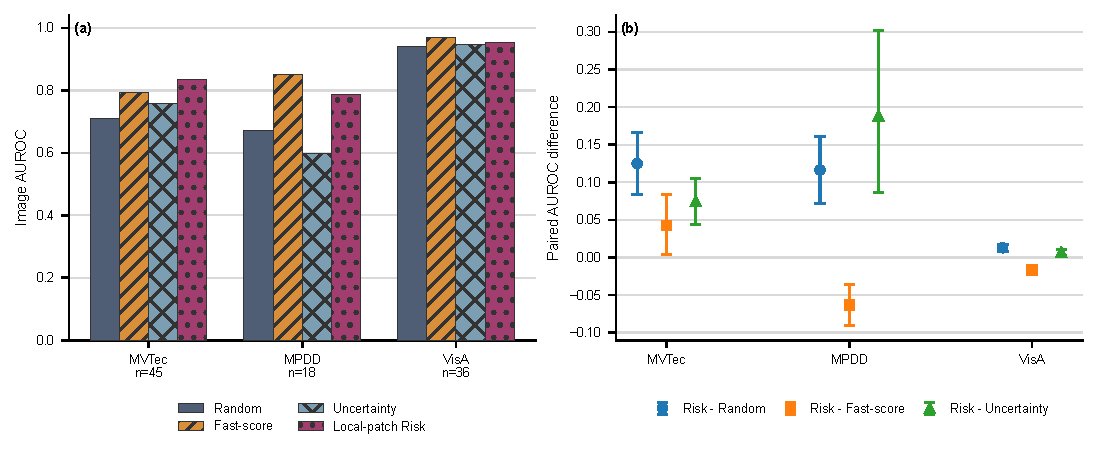
\includegraphics[width=\textwidth]{figures/canonical_v3/fig_canonical_v3_strong_routing.pdf}
\caption{Matched 25\% routing comparison under the offline strict quota. Panel (a) shows mean image-level AUROC by dataset. Panel (b) shows paired AUROC differences between local-patch risk and each routing baseline, with fixed-seed 95\% paired bootstrap intervals. Labels report category-seed rows, not independent industrial datasets}\label{fig:cross-effects}
\end{figure*}

\subsection{Full-budget detector references}

The full detector is the accuracy reference. Its pooled image-level AUROC on MVTec was 0.9392, compared with 0.8343 for the strict 25\% local-patch route and 0.7094 for matched-random. Local-patch routing improves the use of a limited budget, but it does not reach the accuracy obtained when every image uses the full detector.

A PaDiM-style baseline achieved pooled AUROC 0.8982 and Recall@5\%FPR 0.6544 over 45 MVTec category-seed units. Under the reported approximation, a patch-level farthest-point coreset detector reached AUROC 0.9433 and Recall@5\%FPR 0.7847. Both are full-budget references with higher absolute detection quality. Their purpose here is contextual; they do not test whether local-patch risk selects better fallback cases than matched-random at the same count.

\subsection{Budget sensitivity}

On MVTec AD, local-patch risk improves allocation at 10\%, 25\% and 50\% budgets under the same three-seed protocol. Each point contains 45 category-seed units (15 categories $\times$ 3 seeds), with identical fallback counts across policies. Figure~\ref{fig:budget} reports paired differences from matched-random. The AUROC difference rises from +0.1145 (95\% CI [0.0821, 0.1484]) at 10\% to +0.1249 ([0.0837, 0.1659]) at 25\% and +0.1589 ([0.1226, 0.1954]) at 50\%. Recall@5\%FPR follows the opposite pattern, decreasing from +0.4981 ([0.3940, 0.5977]) to +0.3877 ([0.2916, 0.4792]) and +0.2479 ([0.1834, 0.3110]). All three budget points remain positive, so the result is not confined to the 25\% setting.

\begin{figure*}[t]
\centering
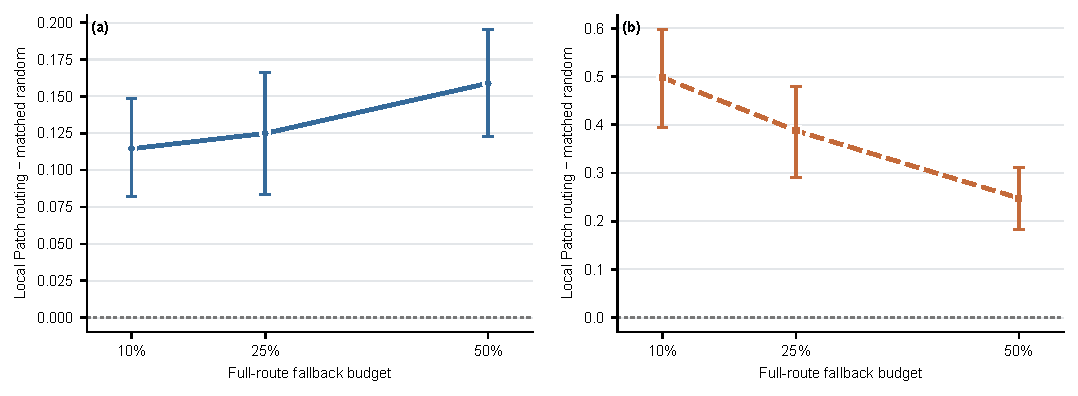
\includegraphics[width=\textwidth]{figures/Fig3_budget_sensitivity.pdf}
\caption{MVTec budget sensitivity under the three-seed strict-quota protocol. Panel (a) shows the paired image-level AUROC difference between local-patch risk and matched-random at 10\%, 25\% and 50\% fallback budgets. Panel (b) shows the corresponding Recall@5\%FPR difference. Error bars are fixed-seed 95\% paired bootstrap intervals over 45 category-seed units}\label{fig:budget}
\end{figure*}

\subsection{Deployment boundary}

Figure~\ref{fig:latency-audit} gives a separate MVTec batch-one CUDA audit. At the same nominal 25\% fallback rate, mean/P95 latency is 5.1899/6.7302 ms for Risk and 3.6269/4.0860 ms for Full. Because these measurements are not paired with the accuracy rows, they define a deployment limitation rather than an efficiency gain.

\begin{figure*}[t]
\centering
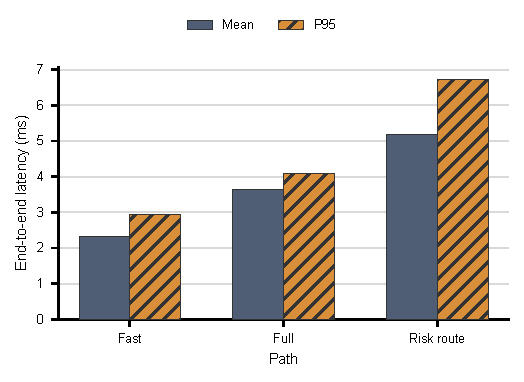
\includegraphics[width=\textwidth]{figures/canonical_v2/fig_canonical_v2_latency_audit.pdf}
\caption{Separate MVTec batch-one CUDA latency audit at nominal 25\% fallback. Measurements cover 15 categories and 6,000 images, with CUDA synchronization and 20 repetitions per cached image. The audit is not paired with the accuracy rows and therefore does not establish deployment efficiency}\label{fig:latency-audit}
\end{figure*}

\subsection{Exploratory analyses (supplementary)}

The canonical 25\% result excludes the analyses below. MVTec budget sensitivity at 10\%, 25\% and 50\% appears in the preceding subsection. Online-prefix routing depends on configuration: the MVTec audit shows a modest positive AUROC change, while VisA has negative low-FPR recall at batch 32. The conformal threshold is only a stress test because its realized fallback rate drifts from the target. The evidence therefore supports offline strict-quota allocation, not online-prefix performance or robustness to distribution shift.

In the MVTec seed-17 ablation, the 1\%, 5\% and 10\% aggregation fractions produced similar AUROC differences from matched-random. The main analysis retains 5\% because that value was fixed before the formal comparison.

\section{Discussion}\label{sec:discussion}

With a fixed number of expensive evaluations, local-patch ranking allocates them better than random selection and the nearest-patch-distance dispersion signal. The comparison uses matched controls on three industrial datasets and three seeds at an offline strict 25\% quota. The gain is small on VisA, and the fast detector's own score works better on MPDD and VisA.

PatchCore and the full local path remain more accurate because they apply the expensive feature path to every image. The result concerns allocation quality rather than detector quality. This distinction is useful when only a fixed number of images can be escalated, but it leaves end-to-end deployment performance unresolved.

Several limitations remain. Fast-score is a better allocation signal on MPDD and VisA, which rules out a general advantage for local-patch risk. Batch-one sequential P95 latency is also higher than Full because the probe runs before selected samples enter the full path. Online behaviour and the conformal diagnostic vary with configuration and do not guarantee a fixed budget. The patch-coreset implementation is a controlled approximation of the standard reduction procedure, and learned uncertainty gatekeepers were not included as fully matched baselines. Finally, the formal evaluation uses established public benchmarks rather than the newly released ISP-AD screen-printing benchmark, which contains weakly contrasted defects \cite{krassnig2026isp}. Category-seed is the statistical unit, so category-level counts do not constitute independent evidence for every industrial class.

Further work should test shared feature computation and an independently trained uncertainty model. A multi-budget, multi-seed study with full-category deployment audits could use a preregistered P95 budget, while shift-aware calibration could control allocation rate and low-FPR recall together. Such experiments would test whether the allocation effect survives changes to the feature path and deployment protocol.

\section{Conclusion}\label{sec:conclusion}

At an offline strict 25\% fallback quota, local-patch risk improves image-level AUROC over equal-count random selection and dispersion uncertainty on MVTec AD, MPDD and VisA. The MVTec advantage over random selection also persists at 10\% and 50\% budgets. Fast-score performs better on MPDD and VisA, so local-patch risk remains a dataset-dependent allocation policy rather than a generally superior one. Because every category-seed unit receives the same number of expensive evaluations, the comparison isolates the allocation rule from the fallback budget. These findings do not extend to full-detector accuracy, lower single-sample latency or universal online robustness.

\section{Methods}\label{sec:methods}

\subsection{Implementation details}
All experiments use features from an ImageNet-pretrained ResNet-18. The fast path takes $128\times128$ inputs and layer-2 features, while the full path takes $224\times224$ inputs and layer-3 patch features. Memory banks contain features from normal training images only. The local probe uses the top 5\% aggregation fraction. Formal experiments use fixed seeds 5, 17 and 29. For each run, the evaluation code writes category, seed, budget, realized fallback rate, AUROC, Recall@5\%FPR and latency to JSON.

\subsection{Latency measurement}
CUDA latency measurements use explicit synchronization, one warm-up and repeated evaluation of cached images. We report mean and P95 latency for the Fast, Full and Risk (probe-plus-Full) paths. Repetitions measure a system property and are not independent units in the accuracy bootstrap.

\subsection{Statistical analysis}
For each dataset and budget, comparisons are paired at the category-seed level. The bootstrap samples these units with replacement and calculates the route difference for every replicate. We report two-sided 95\% confidence intervals. Interpretation considers whether the paired interval excludes zero as well as the direction and size of the difference. Positive category counts are descriptive.

\subsection{Ethics and reproducibility}
This study uses public image datasets and includes no human participants, animals or personally identifiable information. The reference list cites the dataset sources. The public project repository contains the analysis materials and will host the submission-matched split protocol, figure source data, derived result tables and evaluation scripts.

\backmatter

\section*{Acknowledgements}
The authors thank the MVTec AD, MPDD and VisA maintainers for providing the benchmark datasets.

\section*{Statements and Declarations}
\textbf{Funding.} This study and manuscript received no funding.

\textbf{Competing interests.} The authors have no relevant financial or non-financial competing interests.

\textbf{Ethics approval and consent to participate.} Not applicable. The study uses public benchmark datasets and includes no human or animal participants.

\textbf{Consent for publication.} Not applicable.

\textbf{Data availability.} MVTec AD is available from \url{https://www.mvtec.com/research-teaching/datasets/mvtec-ad}, MPDD from \url{https://github.com/stepanje/MPDD}, and VisA from the Registry of Open Data on AWS at \url{https://registry.opendata.aws/visa/}. The supplementary analyses and derived summary tables are included with the Supplementary Information, while category-seed result tables and figure source data are maintained in the project repository at \url{https://github.com/cdhuangjin/fixed-budget-patch-routing}.

\textbf{Code availability.} The evaluation scripts, configuration files and route definitions will be made available in a submission-matched release at \url{https://github.com/cdhuangjin/fixed-budget-patch-routing}.

\textbf{Author contributions.} J.H. designed the study, implemented the analysis, ran the experiments and drafted the manuscript. Q.G. reviewed the experiments and contributed to interpretation and revision. Both authors approved the final manuscript.

\bibliography{references}

\end{document}
